%----------------------------------------------%
%                                              %
% Title:  Linux device drivers explained       %
% Author: Giuseppe Calderaro                   %
% Date:   29th October 2009                    %
%                                              %
%----------------------------------------------%

% Latex document class
\documentclass{beamer}
\usepackage{beamerthemeshadow}
\usepackage{listings}
\usepackage{xcolor}
\lstset{language=C}
\setbeamertemplate{navigation symbols}{}
\usetheme{Berkeley}
\beamersetuncovermixins{\opaqueness<1>{25}}{\opaqueness<2->{15}}

% Document start
\begin{document}
\title{Linux Device Drivers explained}
\author{Giuseppe Calderaro}
\institute[http://www.imgtec.com/]{Imagination technologies ltd.}
\date{29th October 2009}

% Slide: 1
\frame{
  \titlepage
  \begin{figure}
    
\includegraphics[scale=0.20]{emacs.eps}
  \end{figure} 
}

%% LINUX SYSTEM ARCHITECTURE
% Slide: 2
\section{Linux system architecture}
\subsection{Linux system architecture}
\frame{\frametitle{Linux system architecture}
  \begin{columns}
    \begin{column}{10cm}
      \begin{figure}
        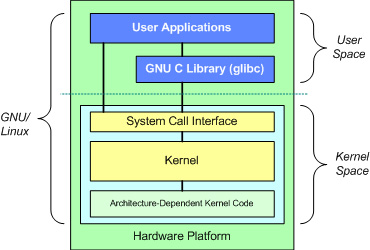
\includegraphics[scale=0.75]{arch1.eps}
        \caption{Linux system architecture}
      \end{figure}
    \end{column}
  \end{columns}
}

% Slide: 3
\subsection{Linux kernel architecture}
\frame{\frametitle{Linux kernel architecture}
  \begin{columns}
    \begin{column}{3cm}
      \begin{figure}
        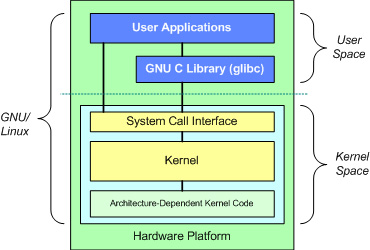
\includegraphics[scale=0.35]{arch1.eps}
        \caption{\tiny{Linux system architecture}}
      \end{figure}
    \end{column}
    \begin{column}{7cm}
      \begin{figure}
        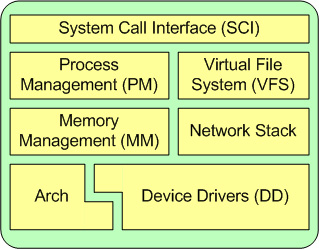
\includegraphics[scale=0.65]{arch2.eps}
        \caption{Linux kernel architecture}
      \end{figure}     
    \end{column}
  \end{columns}
}

\subsection{Linux kernel architecture detailed}
\frame{\frametitle{... in detail}
  \includegraphics[scale=0.50]{kernel.eps}
}

%% BUILDING AND RUNNING MODULES
% Slide: 4
\section{Building and running modules}
\subsection{A polite module...}
\frame{\frametitle{A polite module...}
  \makebox{
    \scriptsize{
      \lstinputlisting{example.c}
    }
  }
}

% Slide: 5
\subsection{...and his Makefile}
\frame{\frametitle{...and his Makefile}
  \makebox{
    \scriptsize{
      \lstinputlisting{Module_Makefile}
    }
  }
}

%% DEBUGGING TECHNIQUES
% Slide: 6->8
\section{Debugging techniques}
\subsection{printk}
\frame{\frametitle{printk}
  \begin{itemize}
    \item<1-> printf(''I am printf!'');
    \item<2-> printk(KERN\_INFO ''I am printk!'');
    \item<3-> printf prototype: int printf(const char *format, ...);
    \item<3-> printk prototype: int printk(const char *fmt, ...);
  \end{itemize}
}

% Slide: 9->10
\subsection{Log level values}
\frame{\frametitle{Log level values}
  \begin{itemize}
    \item<1-> \lstinputlisting{kernel_1line.h}
    \item<2-> \lstinputlisting{kernel_2line.h}
  \end{itemize}
}

% Slide: 11
\frame{\frametitle{Log level values}
  \makebox{
    \scriptsize{
      \lstinputlisting{kernel.h}
    }
  }
}

% Slide: 12->14
\subsection{mmm... proc... what's that?!?}
\frame{\frametitle{mmm... proc... what's that?!?}
  \begin{itemize}
  \item<1->{
    [giuseppe@wopr ~]\$ cat /proc/sys/kernel/printk\\
    3\hspace{1.5cm}4\hspace{1.5cm}1\hspace{1.5cm}7
  }
  \item<2-> Current Default Minimum Boottime
  \item<3-> echo 8 $>$ /proc/sys/kernel/printk
  \item<3-> if the value is set to 8, all messages, including debugging ones, are displayed.
  \end{itemize}
}

% Slide: 15
\subsection{Other debugging techniques}
\frame{\frametitle{Other debugging techniques}
  \begin{itemize}
    \item Use the /proc filesystem
    \item Use ioctl method
    \item Debugging by watching (strace, ltrace)
    \item Oops messages (continues...)
    \item gdb vmlinux /proc/kcore
    \item kdb kernel debugger
    \item kgdb kernel debugger (in vanilla)
    \item User mode linux (!?!)
    \item Linux Trace Toolkit
    \item Kernel probes (good good)
    \item ice kernel debugger (waited for 4891AD)
  \end{itemize}
}

% Slide: 16
\subsection{OOOOOOOPS!}
\frame{\frametitle{OOOOOOOPS!}
  \tiny{
    \lstinputlisting{oops.txt}
  }
}

% Slide: 17
\section{Concurrency and Race conditions}
\subsection{Semaphores and mutexes}
\frame{\frametitle{Semaphores and mutexes}
  \scriptsize{
    \lstinputlisting{semaphores.txt}
  }  
}

% Slide: 18
\subsection{Reader/writer Semaphores}
\frame{\frametitle{Reader/writer semaphores}
  \tiny{
    \lstinputlisting{rwsem.txt}
  }    
}

% Slide: 19
\subsection{Completions}
\frame{\frametitle{Comple...}
  A common pattern in kernel programming involves initiating some activity outside of
  the current thread, then waiting for that activity to complete.
  \scriptsize{
    \lstinputlisting{completions1.txt}
  }
}

% Slide: 20
\subsection{Completions}
\frame{\frametitle{...tions}
  \scriptsize{
    \lstinputlisting{completions2.txt}
  }
}

% Slide: 21
\subsection{Spinlocks and...}
\frame{\frametitle{Spinlocks and...}
  \tiny{
    \lstinputlisting{spinlocks.txt}
  }  
}

% Slide: 22
\subsection{...Atomic Context!}
\frame{\frametitle{...Atomic Context!}
  In atomic context (interrupt context, softirq context)\\
  YOU CAN'T:
  \begin{itemize}
    \item Schedule
    \item Sleep
    \item Use semaphores (they could go to sleep)
  \end{itemize}
  and\\
  \begin{center}
    YOU MUST USE SPINLOCKS!\\
  \end{center}
  Otherwise:\\
  \begin{center}
    BUG: scheduling while atomic\\
    kernel panic, not syncing. Aiiie, killing interrupt handler...
  \end{center}
}

% Slide: 23
\subsection{Reader/Writer Spinlocks}
\frame{\frametitle{Reader/Writer Spinlocks}
  \tiny{
    \lstinputlisting{rwspinlocks.txt}
  }
}

% Slide: 24
\subsection{Lock-Free Algorithms}
\frame{\frametitle{Lock-Free Algorithms}
  \begin{itemize}
  \item Circular buffers
  \item Atomic variables
  \item Bit operations
  \item seqlocks (continues...)
  \item Read-Copy update (continues...)
  \end{itemize}
}

% Slide: 25
\subsection{seqlocks}
\frame{\frametitle{seqlocks}
  Read access works by obtaining an (unsigned) integer sequence value on entry into
  the critical section. On exit, that sequence value is compared with the current value;
  if there is a mismatch, the read access must be retried. As a result, reader code has a
  form like the following:

  \scriptsize{
    \lstinputlisting{seqlocks.txt}
  }
}

% Slide: 26
\subsection{Read-Copy-Update}
\frame{\frametitle{Read-Copy-Update}  
  \scriptsize{
    \lstinputlisting{rcu.txt}
  }
  \tiny{
    \lstinputlisting{rcu_link.txt}
  }
}

% Slide: 27
\section{Allocating memory}
\subsection{The real story of kmalloc}
\frame{\frametitle{The real story of kmalloc}
  \scriptsize{
    \lstinputlisting{kmalloc.txt}
  }
  \begin{table}
    \scriptsize{\caption{Flags:}}
    \begin{tabular}{c c}      
      \hline
      Allocation priorities & Allocation flags\\
      \hline  
      GFP\_ATOMIC & \_\_GFP\_DMA\\
      GFP\_KERNEL & \_\_GFP\_HIGHMEM\\
      GFP\_USER & \_\_GFP\_COLD\\
      GFP\_HIGHUSER & \_\_GFP\_NOWARN\\
      GFP\_NOIO & \_\_GFP\_HIGH\\
      GFP\_NOFS & \_\_GFP\_REPEAT\\    
      & \_\_GFP\_NOFAIL\\
      & \_\_GFP\_NORETRY\\
    \end{tabular}
  \end{table}
}

% Slide: 28
\subsection{Lookaside caches}
\frame{\frametitle{Lookaside caches}
  \scriptsize{
    A device driver often ends up allocating many objects of the same size, over and over.
  }
  \tiny{
    \lstinputlisting{caches.txt}
  }
  
}

% Slide: 29
\subsection{Memory pools}
\frame{\frametitle{Memory pools}
  There are places in the kernel where memory allocations cannot be allowed to fail.
  As a way of guaranteeing allocations in those situations, the kernel developers created
  an abstraction known as a memory pool (or ''mempool''). A memory pool is
  really just a form of a lookaside cache that tries to always keep a list of free memory
  around for use in emergencies.
}

% Slide: 30
\subsection{get_free_page and co}
\frame{\frametitle{get\_free\_page and co}
  \tiny{
    \lstinputlisting{get_free_page.txt}
  }
}

% Slide: 31
\subsection{vmalloc and friends}
\frame{\frametitle{vmalloc and friends}
  \scriptsize{
    vmalloc allocates a contiguous memory region in the virtual address space.\\
    Although the pages are not consecutive in physical memory\\
    the kernel sees them as a contiguous range of addresses.\\
    vmalloc is described here because it is one of the fundamental Linux memory allocation mechanisms.\\
    We should note, however, that use of vmalloc is discouraged in most\\
    situations. Memory obtained from vmalloc is slightly less efficient to work with,\\
    and, on some architectures, the amount of address space set aside for vmalloc is relatively small.\\
    Code that uses vmalloc is likely to get a chilly reception if submitted for\\
    inclusion in the kernel. If possible, you should work directly with individual pages\\
    rather than trying to smooth things over with vmalloc.
  }
}

% Slide: 32
\subsection{vmalloc api}
\frame{\frametitle{vmalloc api}
  \scriptsize{
    \lstinputlisting{vmalloc.txt}
  }
}

% Slide: 33
\section{Communicating with hardware}
\subsection{Communicating with hardware}
\frame{\frametitle{Communicating with hardware}
  \tiny{
    \lstinputlisting{devmem.txt}
  }
}

% Slide: 34
\subsection{Installing an interrupt handler}
\frame{\frametitle{Installing an interrupt handler}
  \tiny{
    \lstinputlisting{interrupt.txt}
  }
  \begin{table}
    \scriptsize{\caption{Flags:}}
    \begin{tabular}{c}      
      \hline
      Interrupt flags:\\
      \hline  
      SA\_INTERRUPT\\
      SA\_SHIRQ\\
      SA\_SAMPLE\_RANDOM\\
    \end{tabular}
  \end{table}
}

% Slide: 35
\subsection{Top and bottom halves}
\frame{\frametitle{Top and bottom halves}
  One of the main problems with interrupt handling is how to perform lengthy tasks\\
  within a handler.\\
  In the typical scenario, the top half saves device data to a device-specific buffer,\\
  schedules its bottom half, and exits: this operation is very fast.\\
  The bottom half then performs whatever other work is required,\\
  such as awakening processes, starting up another I/O operation, and so on.\\
  This setup permits the top half to service a new interrupt while the bottom half is still working.
}

% Slide: 36
\section{Kernel data types}
\subsection{Kernel data types}
\frame{\frametitle{Kernel data types}
  \scriptsize{
    \begin{table}
      \begin{tabular}{c c c c c c c c c c c}      
        \hline
        arch    & char & short & int & long & ptr & long long & u8 & u16 & u32 & u64\\
        \hline  
        i386    & 1 & 2 & 4 & 4 & 4 & 8 & 1 & 2 & 4 & 8\\
        alpha   & 1 & 2 & 4 & 8 & 8 & 8 & 1 & 2 & 4 & 8\\
        armv4l  & 1 & 2 & 4 & 4 & 4 & 8 & 1 & 2 & 4 & 8\\
        ia64    & 1 & 2 & 4 & 8 & 8 & 8 & 1 & 2 & 4 & 8\\
        m68k    & 1 & 2 & 4 & 4 & 4 & 8 & 1 & 2 & 4 & 8\\
        mips    & 1 & 2 & 4 & 4 & 4 & 8 & 1 & 2 & 4 & 8\\
        ppc     & 1 & 2 & 4 & 4 & 4 & 8 & 1 & 2 & 4 & 8\\
        sparc   & 1 & 2 & 4 & 4 & 4 & 8 & 1 & 2 & 4 & 8\\
        sparc64 & 1 & 2 & 4 & 4 & 4 & 8 & 1 & 2 & 4 & 8\\
        x86\_64 & 1 & 2 & 4 & 8 & 8 & 8 & 1 & 2 & 4 & 8\\
      \end{tabular}
    \end{table}
  }
}

% Slide: 37
\section{Memory Layout}
\subsection{Memory Layout}
\frame{\frametitle{Memory Layout}
  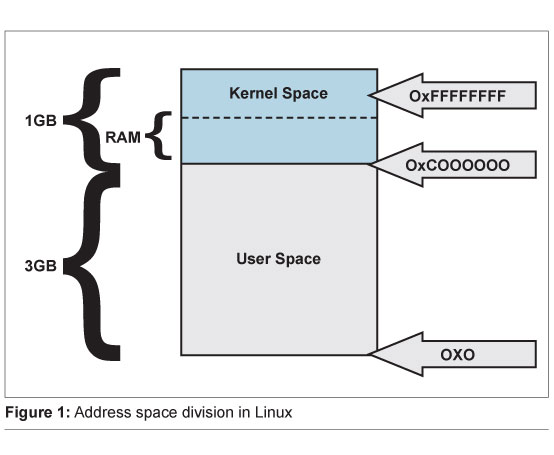
\includegraphics[scale=0.50]{address_div.eps}
}

% Slide: 38
\subsection{Memory Layout}
\frame{\frametitle{Memory UM}
  \includegraphics[scale=0.50]{memory.eps}
}

% Slide: 39
\section{Thanks}
\subsection{Thanks}
\frame{\frametitle{Thanks}
  \begin{center}
    \Huge{\textcolor{red}{typedef is evil!}\\
      Thanks :-)      
    }
  \end{center}
}

% Document end
\end{document}
